\chapter{Combined acceleration and a five-second load pulse}
\textit{Archived October study. All simulations, searches, and checks described below predate this report.}\par

\section{Requested cycle}
Define relative time $\tau=t-60$ s. The shaft-speed target and external load are
\begin{align}
r(\tau)&=9000+200\min(5,\max(0,\tau))\quad\mathrm{rpm},\\
P_L(\tau)&=\begin{cases}0.1P_{\rm ref},&10\le\tau<15,\\0,&\text{otherwise}.\end{cases}
\end{align}
The speed target ramps from 90\% to 100\% in five seconds, then remains at 10000 rpm. A common load is applied at second 10 and removed at second 15. Recovery is recorded through second 25.005. The five-second pulse is programmed as a zero-order-held workspace signal, with interpolation disabled.

The reference is the mean turbine shaft power at settled 10000 rpm from seconds 8--10 of the preceding no-load base-PI run: $P_{\rm ref}=27896.501$ hp. Therefore every controller receives exactly the same pulse amplitude, 2789.650 hp. This is 10\% of that common turbine-power reference, not 10\% of each controller's instantaneous power. Internal compressor power is still present.

The preparation stage begins at 10000 rpm, moves to 9000 rpm during absolute seconds 5--10, and settles before the cycle starts at absolute second 60. All cases use sea-level ISA-zero, Mach-zero conditions. Controller gains remain fixed. All four sensors have a 0.05 s time constant, unity gain, identical limits and initial conditions, and noise disabled. Wiring assertions confirm that each active controller receives the sensor output.

The model sample interval is 0.015 s. The first logged loaded sample is at relative 10.005 s, and the first unloaded sample is at 15.000 s. The programmed event interval is exactly 10--15 s; observed event timing is resolved on the sample grid. All simulations pass the existing model-validity checks.
\section{Comparison definitions}
Error means actual shaft speed minus target, $e_k=N_k-r_k$. Ramp RMSE uses $0\le\tau<5$ s; load/recovery RMSE uses $10\le\tau\le25.005$ s; full-cycle RMSE uses $0\le\tau\le25.005$ s. These are sample-weighted metrics. Scoring the two phases separately prevents the long recovery interval from concealing ramp differences.
\section{Recorded responses}
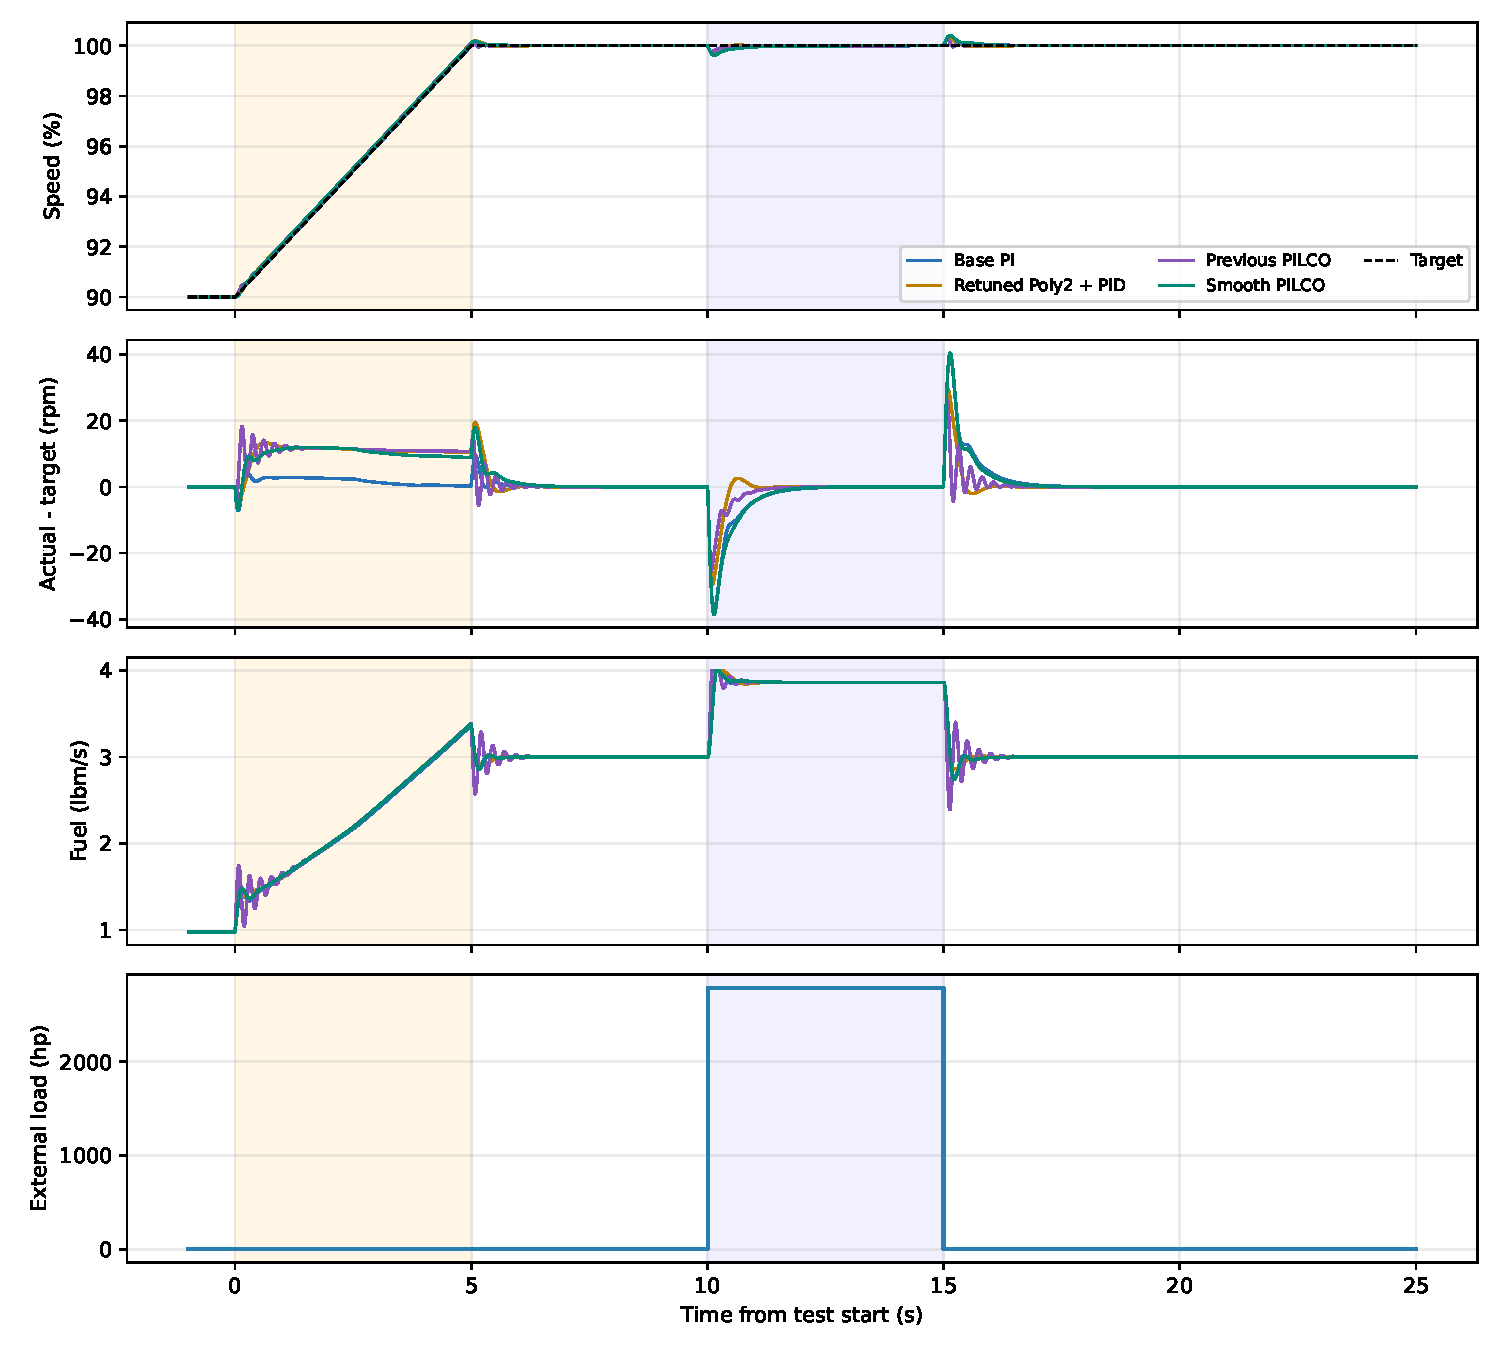
\includegraphics[width=\textwidth,height=.68\textheight,keepaspectratio]{late3_responses.pdf}
Orange shading marks the target ramp; blue shading marks the external-load pulse. These are raw nonlinear simulation traces, with no visual smoothing.
\section{Numerical results}
\begin{center}\small\begin{tabular}{lrrr}\toprule
Controller & Ramp RMSE & Load/recovery RMSE & Full RMSE\\ & rpm & rpm & rpm\\\midrule
Base PI & 2.161 & 6.815 & 5.408 \\
Retuned Poly2 + PID & 10.949 & 4.416 & 6.214 \\
Previous PILCO & 11.224 & 3.393 & 5.745 \\
Smooth PILCO & 10.252 & 6.913 & 7.207 \\
\bottomrule\end{tabular}\end{center}
\begin{center}\small\begin{tabular}{lrrrr}\toprule
Controller & Load peak $|e|$ & Fuel excess TV & Min. surge & Saturation\\
& rpm & lbm/s & \% & \% samples\\\midrule
Base PI & 40.13 & 0.945 & 7.64 & 0.7 \\
Retuned Poly2 + PID & 29.39 & 0.696 & 7.75 & 0.1 \\
Previous PILCO & 26.03 & 4.489 & 7.77 & 0.7 \\
Smooth PILCO & 40.47 & 0.919 & 7.63 & 0.2 \\
\bottomrule\end{tabular}\end{center}
Fuel excess total variation is $\sum|\Delta u|-|u_{\rm end}-u_{\rm start}|$, computed separately over 10--15 s and 15--25.005 s and then summed. It describes excess command movement, not fuel consumption. Minimum surge margin and fuel saturation are evaluated over the full cycle.

The previous and smooth PILCO policies use quadratic setpoint feedforward plus PI feedback. Retuned Poly2 retains its inverse-model/PID implementation; base PI remains the original baseline. No gains, feedforward coefficients or ringing weights were fitted to this combined cycle. These are nominal transfer-test results, not proof of robustness or global superiority. In particular, all controllers share the same sensor dynamics; differences in actual-speed tracking must not be attributed to unequal sensor time constants.
\section{Reproduction and saved outputs}
Run \path{combined_cycle_batch.m} in the existing MATLAB/T-MATS workspace. New models are named \path{GasTurbine_Combined_*.mdl}; earlier studies are preserved. Raw traces, model audit JSON, numerical metrics and the exact protocol are saved under \path{results/pilco_combined_cycle_20261010}. Analysis and video builders are \path{build_combined_cycle.py} and \path{build_combined_video.py}.
